\documentclass{article}
\usepackage{graphicx} % Required for inserting images
\usepackage{amsmath}
\usepackage{microtype}
\usepackage{braket}
\usepackage{amssymb}
\usepackage{pgfplots}
\usepackage{blochsphere}
\usetikzlibrary{angles, quotes}
\pgfplotsset{compat=1.18}

\title{Quantum IS Notes 2}
\author{Aman Meka}
\date{August 2026}

\begin{document}
\maketitle

\setcounter{section}{1}
\section{One Quantum Bit}
\setcounter{subsection}{1}
\subsection{Superposition}
\subsubsection{Zero or One}

Qubit can take two values:
\begin{center}
    \(\ket{0} \text{ or } \ket{1}\)
\end{center}
This is in "\textit{ket}" format.\newline

The bloch sphere is a way to visualize these distinct states.\newline
$\ket{0}$ is the north pole of the bloch sphere.\newline
$\ket{1}$ is the south pole of the bloch sphere.\newline

\subsubsection{Superposition}
A superposition is a combination of $\ket{0} \text{ and } \ket{1}$.\newline

For example:
\begin{displaymath}
    \renewcommand{\arraystretch}{1.8}
    \setlength{\arraycolsep}{15pt} 
    \begin{array}{|c|c|}
        \hline
        \text{Math} & \text{Coords} \\
        \hline
        \frac{1}{\sqrt{2}}(\ket{0}+\ket{1}) & (1,0,0) \\
        \hline
        \frac{1}{\sqrt{2}}(\ket{0}-\ket{1}) & (-1,0,0) \\
        \hline
        \frac{1}{\sqrt{2}}(\ket{0}+i\ket{1}) & (0,-1,0) \\
        \hline
        \frac{1}{\sqrt{2}}(\ket{0}-i\ket(1)) & (0,1,0) \\
        \hline 
    \end{array}
\end{displaymath}
These are commonly represented as:
\begin{center}
    $\ket{+} = \frac{1}{\sqrt{2}}(\ket{0}+\ket{1})$\\
    $\ket{-} = \frac{1}{\sqrt{2}}(\ket{0}-\ket{1})$\\
    $\ket{i} = \frac{1}{\sqrt{2}}(\ket{0}+i\ket{1})$\\
    $\ket{-i} = \frac{1}{\sqrt{2}}(\ket{0}-i\ket(1))$\\
\end{center}
Or another way to represent it is:
\begin{center}
    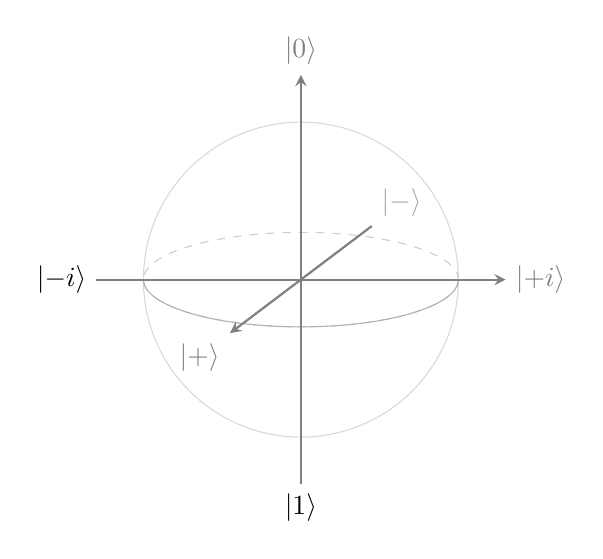
\begin{tikzpicture}[scale=2, >=stealth]
        \coordinate (O) at (0,0);
        \draw[gray!30] (O) circle (1cm);
        \draw[gray!40, dashed] (O) ellipse (1cm and 0.3cm);
        \draw[gray!60] (1,0) arc (0:-180:1cm and 0.3cm);
        \draw[->, thick, gray] (0,-1.3) -- (0,1.3) node[above] {$\ket{0}$};
        \node[below] at (0,-1.3) {$\ket{1}$};
        \draw[->, thick, gray] (-1.3,0) -- (1.3,0) node[right] {$\ket{+i}$};
        \node[left] at (-1.3,0) {$\ket{-i}$};
        \draw[->, thick, gray] (0.45,0.34) -- (-0.45,-0.34) node[below left] {$\ket{+}$};
        \node[above right, gray!70] at (0.45,0.34) {$\ket{-}$};
    \end{tikzpicture}
\end{center}

\end{document}
